\documentclass{beamer}

\usepackage[dutch]{babel}
\usepackage{hyperref}

%\title{Introductie software piraterij}
%\course{}
%\assignment{Warez}
%\assignmenttype{Hacking}
%\authors{Folkert van Verseveld}

%\title[Crisis]{long title} % (optional, only for long titles)
\title{Geschiedenis van Softwarepiraterij}
\author{Folkert van Verseveld}
\institute{Universiteit van Amsterdam}
\date{\today}
\subject{Computer Science}

\begin{document}

\frame{\titlepage}

\begin{frame}
\frametitle{Inhoudsopgave}
%\tableofcontents[currentsection]
\tableofcontents
\end{frame}

\begin{frame}
	\frametitle{Softwarepiraterij}

	\begin{center}
	
\includegraphics[width=\textwidth]{torrentsites.png}
	\end{center}
\end{frame}

\begin{frame}
	\frametitle{Softwarepiraterij}
	%\framesubtitle{Geschiedenis van Warez en technologische ontwikkelingen}
	\framesubtitle{Tijdlijn en ontwikkelingen}

	\begin{itemize}
		\item Warez: voornamelijk electronische software, ook hardware
		\begin{itemize}
			\item De Demoscene
			\item Homebrew
		\end{itemize}
		\item Copy-protection
		\begin{itemize}
			\item Preventie
			\item Omzeilen van Copy-protection en DRM
		\end{itemize}
		% Lijkt me niet nodig dit te bespreken, want daar is vast geen tijd voor...
		% Daarnaast kan het makkelijk even tussendoor genoemd worden wanneer we bespreken hoe legaal softwarepiraterij is...
		%\item Raids en vervolgingen van warez d00dz
	\end{itemize}
\end{frame}

\begin{frame}
	\frametitle{Piraterij is van alle tijden}

	\begin{center}
	
\includegraphics[width=\textwidth]{tape.jpg}
	\end{center}
\end{frame}

\begin{frame}
	\frametitle{Piraterij is van alle tijden}

	\begin{center}
	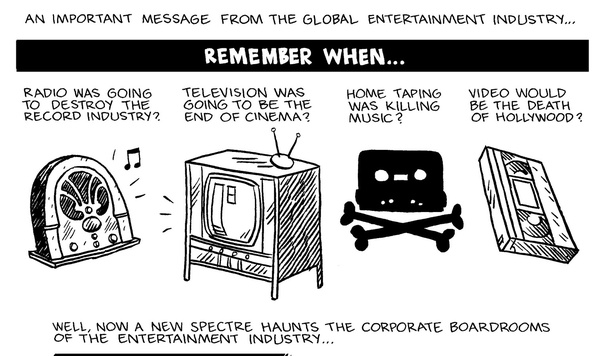
\includegraphics[width=\textwidth]{industry.jpg}
	\end{center}
\end{frame}

\begin{frame}
	%\frametitle{Piraterij is van alle tijden}

	\begin{center}
	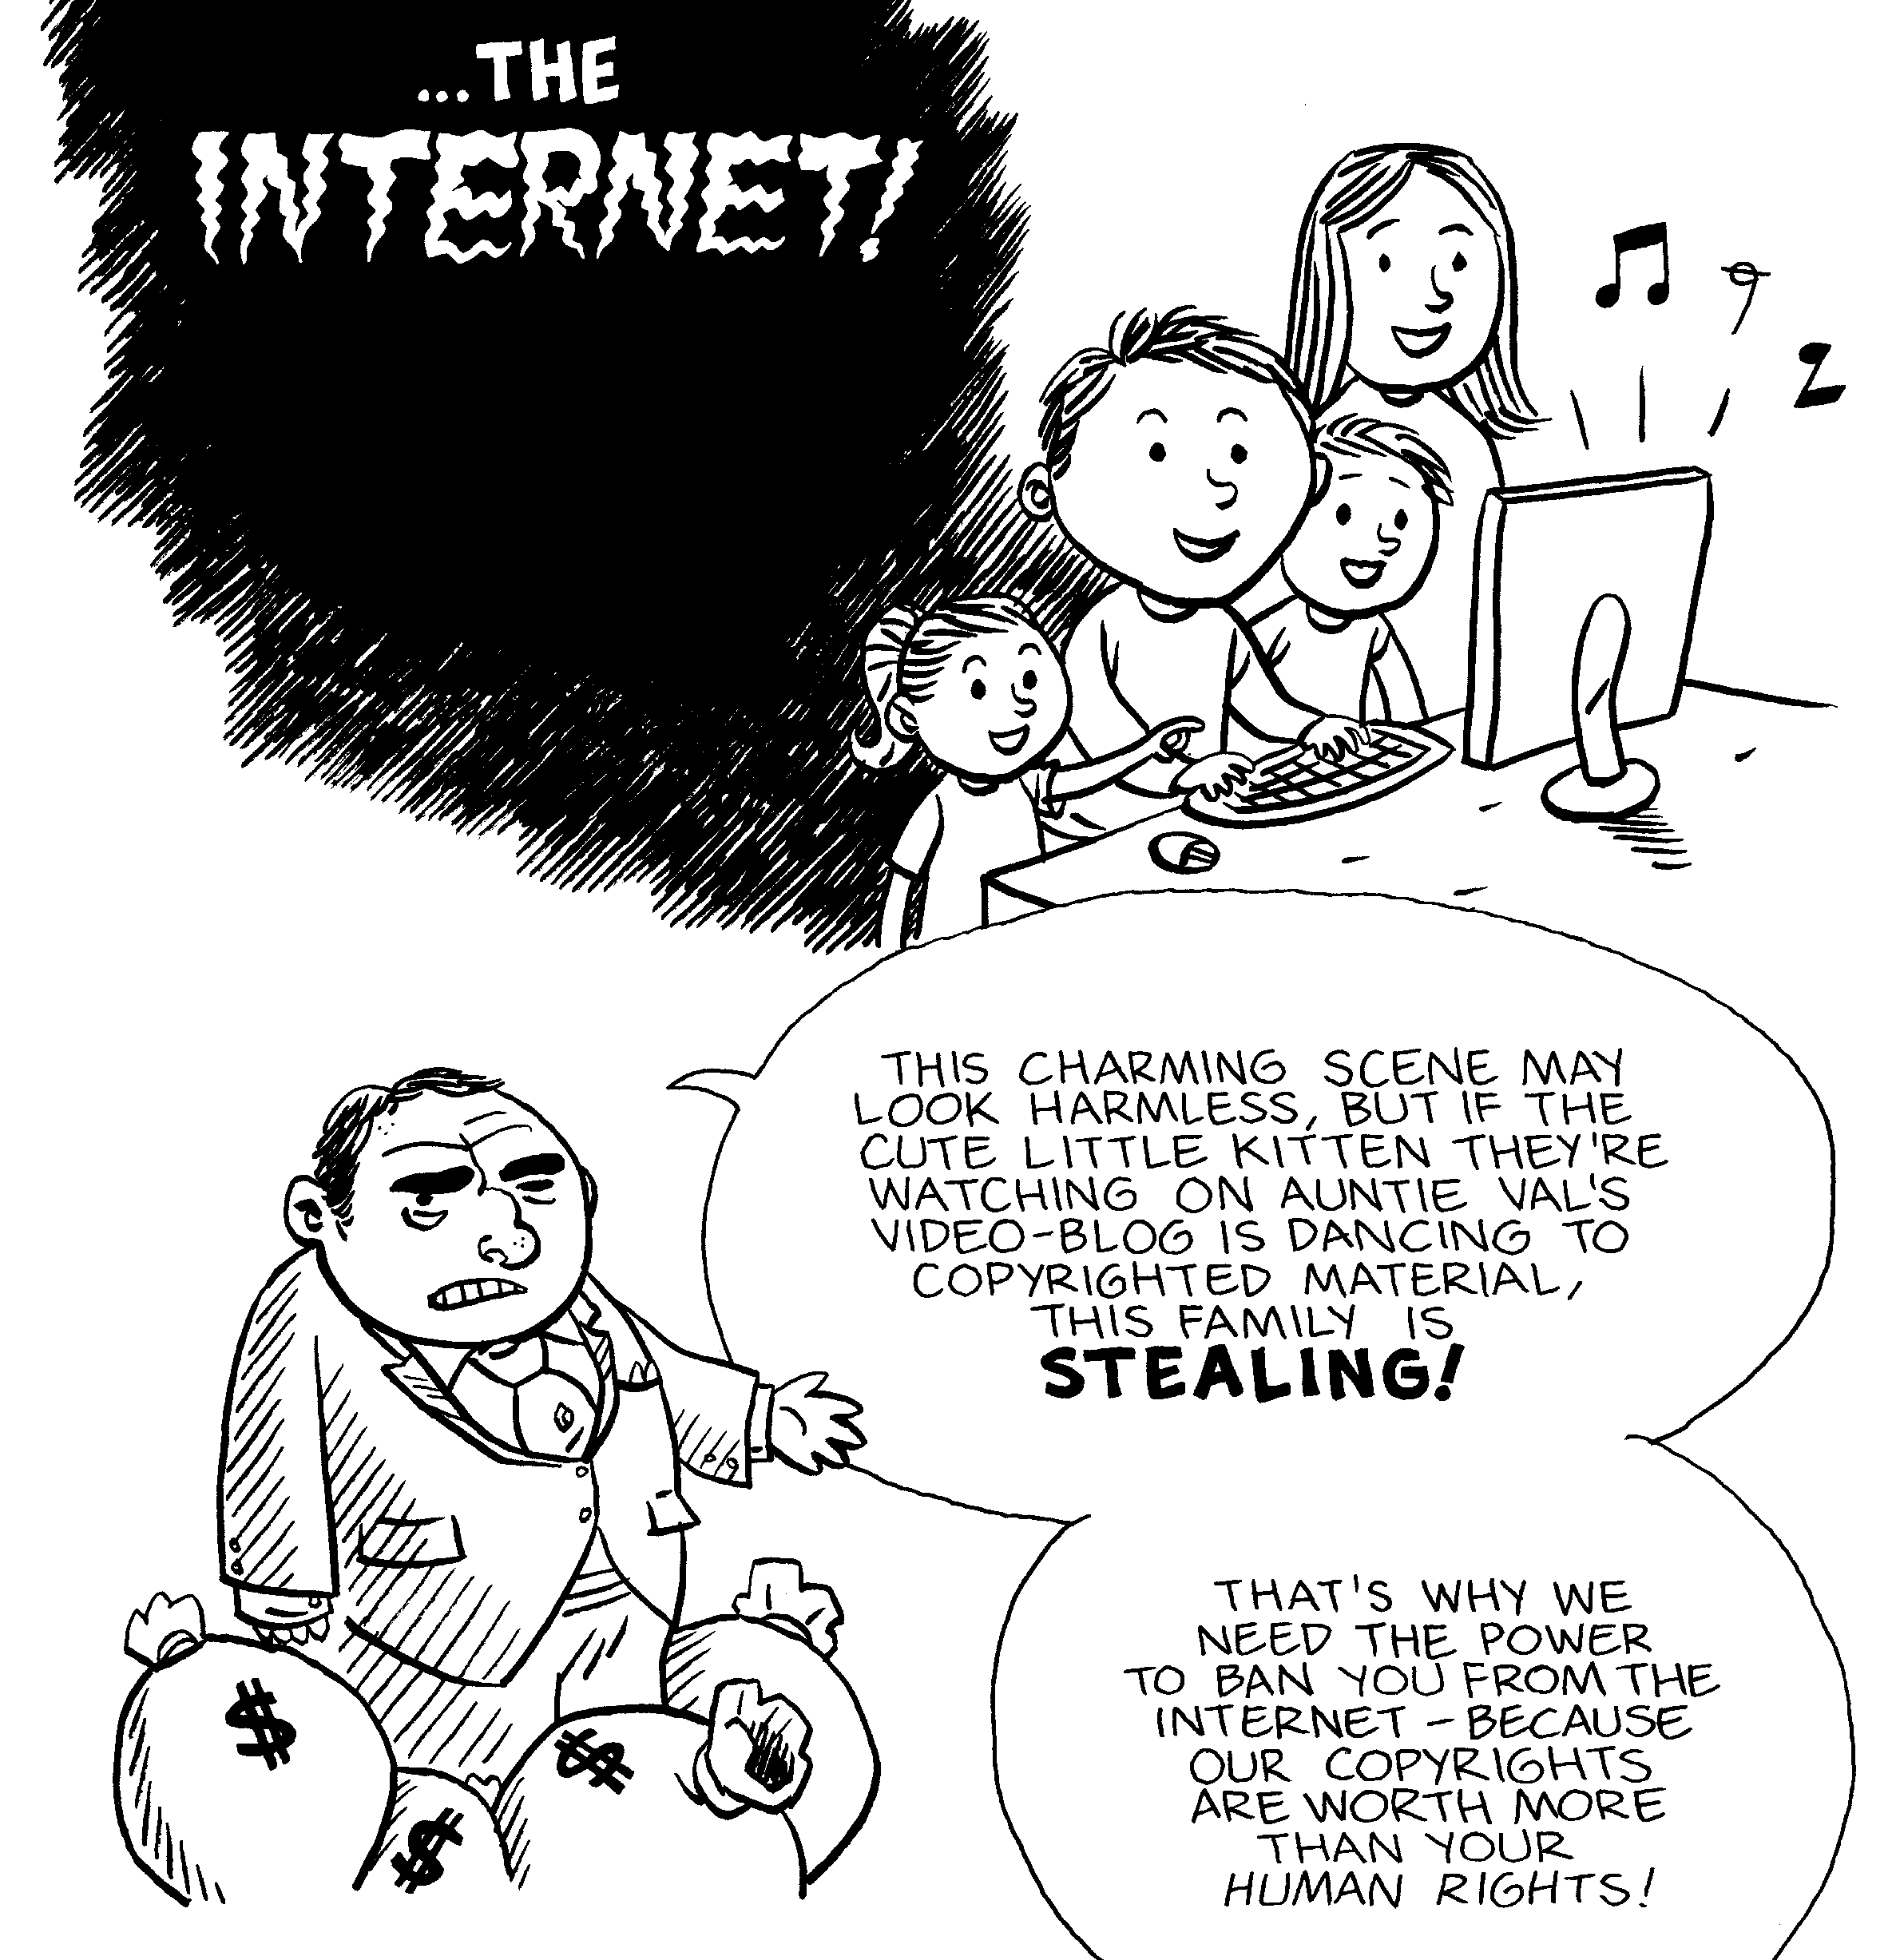
\includegraphics[width=0.85\textwidth]{internet.png}
	\end{center}
\end{frame}

\begin{frame}
	\frametitle{Is piraterij goed of slecht?}

	\begin{itemize}
		\item Meningen verschillen
		\item Wanneer men iets koopt, dan is men de eigenaar ervan(*)
		\item Kopie uitlenen aan kennis/vriend
	\end{itemize}
\end{frame}

\begin{frame}
	\frametitle{Is piraterij goed of slecht?}

	Hoofddoel DRM: uitstellen softwarepiraterij voorbij punt van maximale winst:

	\begin{center}
	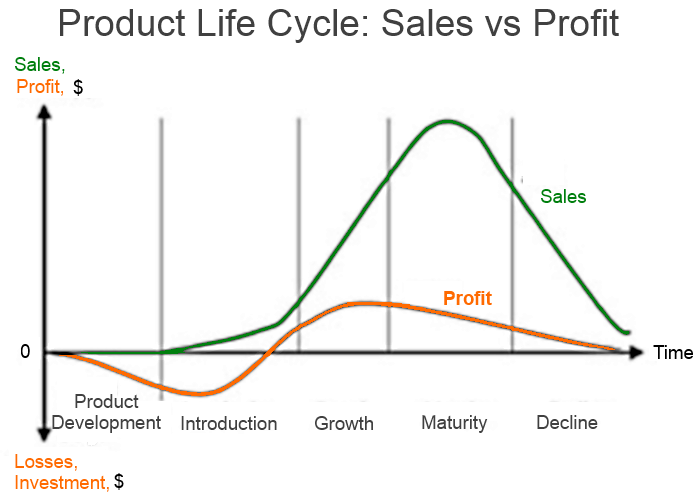
\includegraphics[width=0.85\textwidth]{product_lifecycle.png}
	\end{center}
\end{frame}

\begin{frame}
	\frametitle{Is piraterij goed of slecht?}

	\begin{center}
	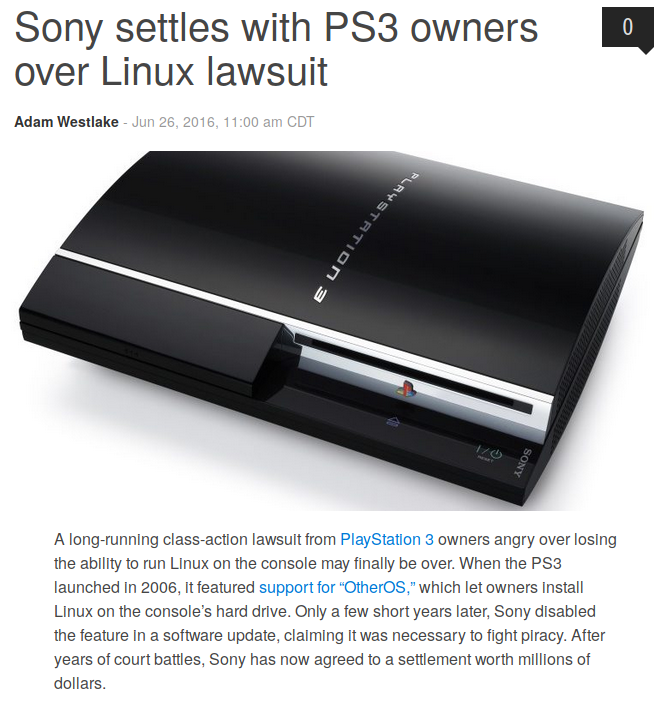
\includegraphics[width=0.75\textwidth]{ps3linux.png}
	\end{center}
\end{frame}

% https://www.youtube.com/watch?v=SMGDW0lOFzc
\begin{frame}
	\frametitle{Is piraterij goed of slecht?}

	\begin{center}
	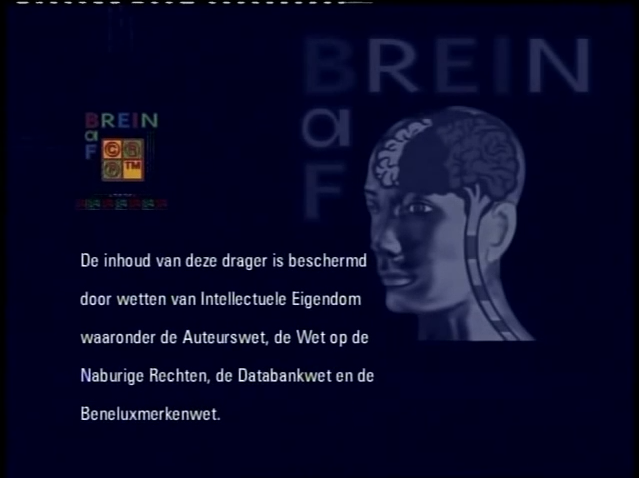
\includegraphics[width=\textwidth]{brein.png}
	\end{center}
\end{frame}

\begin{frame}
	\frametitle{Warez: het ontstaan en verspreiden ervan}

	%Strikeforce: Great Giana Sisters cracktro + trainer
	Moleman 2: The Art of the Algorithms: [50:38, 51:44]
\end{frame}

\begin{frame}
	\frametitle{Warez: cracktro}

	%Strikeforce: Great Giana Sisters cracktro + trainer
	\begin{center}
	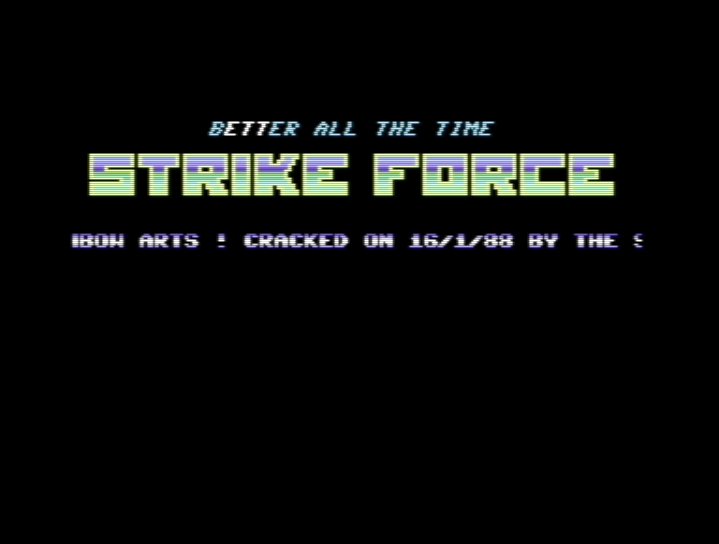
\includegraphics[width=\textwidth]{cracktro_gss.png}
	\end{center}
\end{frame}

\begin{frame}
	\frametitle{Warez: trainer}

	%Strikeforce: Great Giana Sisters cracktro + trainer
	\begin{center}
	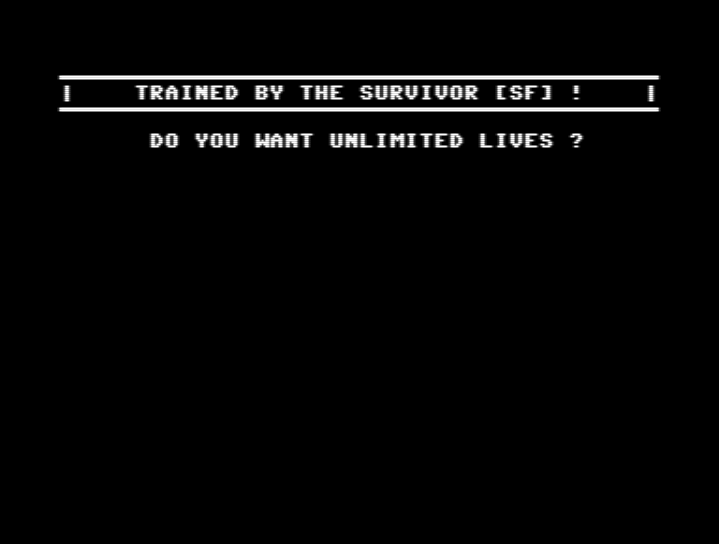
\includegraphics[width=\textwidth]{trainer_gss.png}
	\end{center}
\end{frame}

\begin{frame}
	\frametitle{Warez}

	% TODO
	Tomb Raider Anniversary: hartred cracktro
\end{frame}

\begin{frame}
	\frametitle{Warez}

	SKIDROW: okami
\end{frame}

\begin{frame}
	\frametitle{Warez scene}
	\framesubtitle{Motivatie van verspreiden van warez}

	Behoefte aan kopie\"en maken:
	\begin{itemize}
		\item Backup (opslagmedium was/is onbetrouwbaar)
		\item Beschikbaar maken voor mensen die het niet kunnen kopen
		\begin{itemize}
			\item Niet vanwege prijs, maar uitgever verkoopt niet in het land/de regio
		\end{itemize}
		\item Tegenwoordig: slechte end of life support en verwijderen DRM
	\end{itemize}
\end{frame}

\begin{frame}
	\frametitle{Opslagmedia}

	\begin{center}
	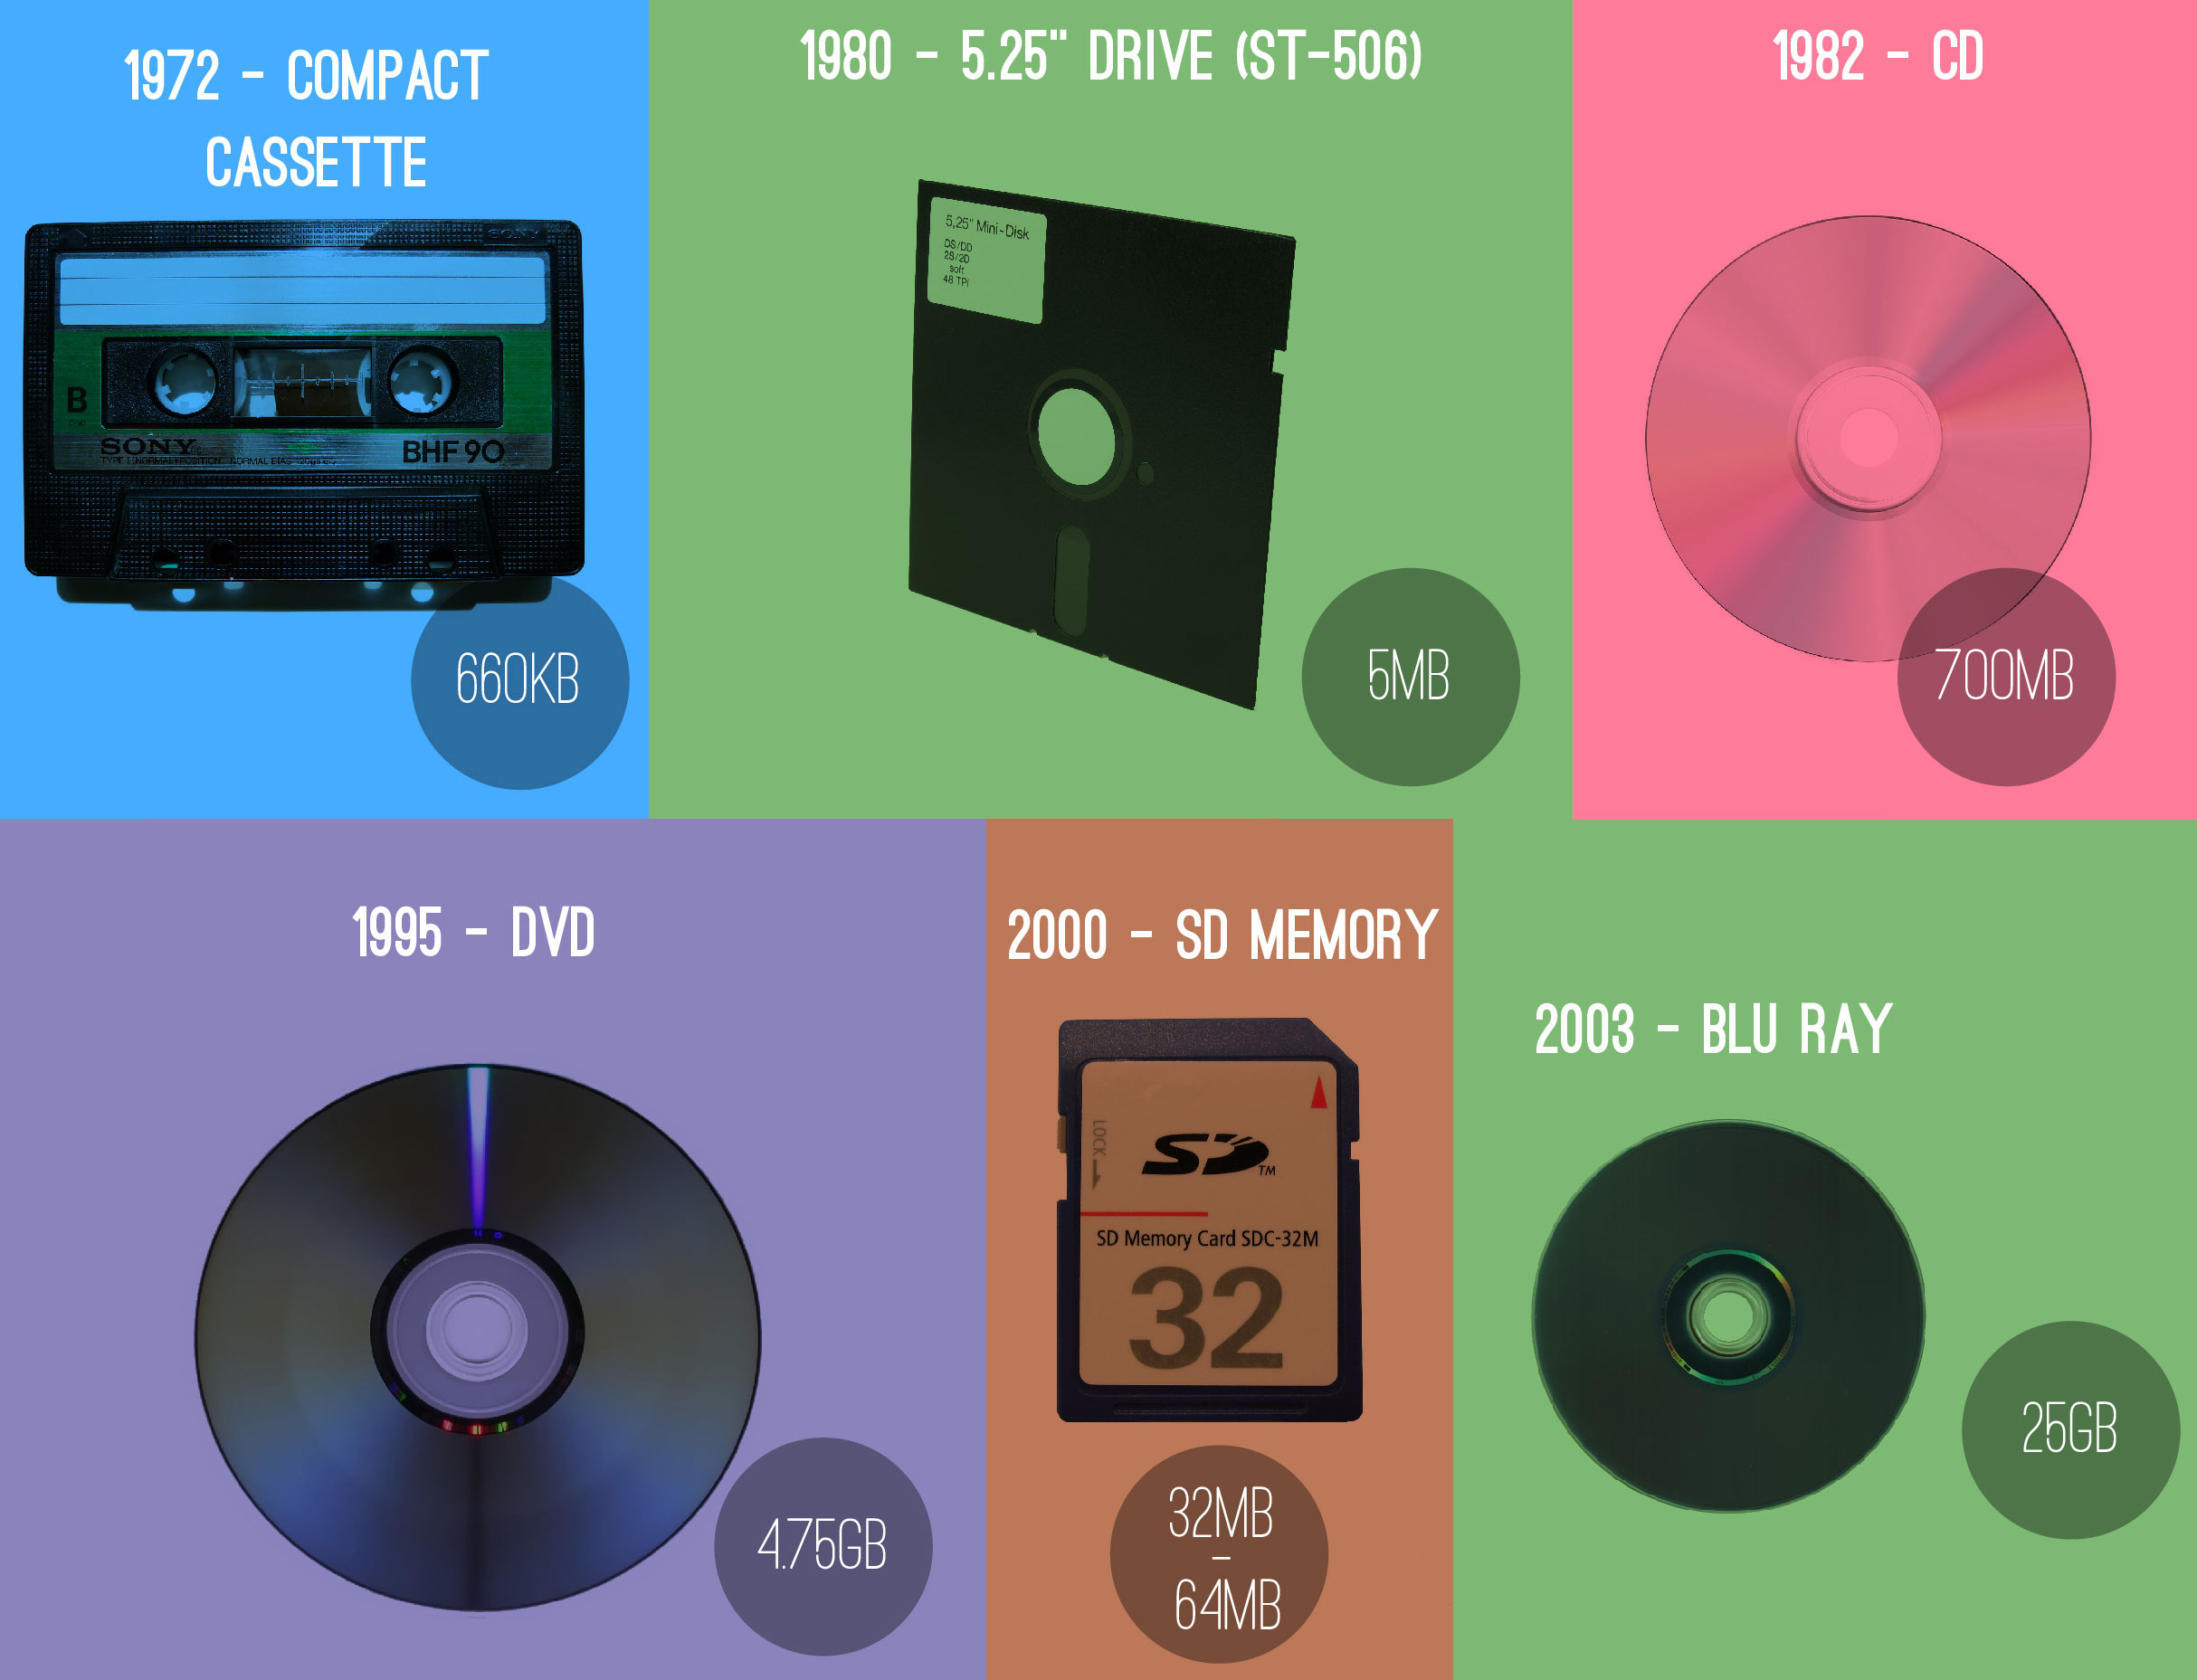
\includegraphics[width=0.8\textwidth]{media.png}
	\end{center}
\end{frame}

\section{Warez}

\begin{frame}
	\frametitle{Warez scene}
	\framesubtitle{Geschiedenis in een notendop}

	\begin{itemize}
		\item Warez scene ontstond voordat het internet bestond
		\item Telefoonlijnen waren het communicatiemiddel
		\item Tweede groeispeurt met komst van commerci\"ele internet
		\item Torrents!
	\end{itemize}
\end{frame}

\begin{frame}
	\frametitle{Warez-groepen}

	\begin{itemize}
		\item CODEX
		\item CONSPIR4CY
		\item FAiRLiGHT
		\item Razor 1911
		\item SKIDROW
		\item \dots
	\end{itemize}
\end{frame}

\begin{frame}
	\frametitle{Warez scene - Anatomie vroeger}

	\begin{itemize}
		% TODO zijn swappers nou de couriers?
		% swappers verspreiden de warez, dus couriers
		\item Release groups maken warez (zgn. Warez d00dz)
		\item Copyparties hosten warez (organizers)
		\item Couriers verspreiden warez (swappers)
		\item Opslagmedium werd aan gebruikers verstrekt of naar opgestuurd
		\item Lokale couriers/vrienden verspreiden warez verder
	\end{itemize}
\end{frame}

\begin{frame}
	\frametitle{Warez scene - Anatomie nu}

	\begin{itemize}
		\item Release groups maken warez (zgn. Warez d00dz)
		\item Topsites hosten warez (Vroeger BBS, nu `darkweb' sites)
		\item Couriers verspreiden warez naar publiek (sysops)
		\item Sites verspreiden torrents naar gebruikers (torrent announcers)
		\item Leechers verspreiden data via peer-to-peer-netwerken
	\end{itemize}
\end{frame}


%\begin{frame}
%	\frametitle{Motivatie van warez-groepen}
%
%	Behoefte aan kopie\"en maken:
%	\begin{itemize}
%		\item Backup (opslagmedium was/is onbetrouwbaar)
%		% later: slechte end of life support (en DRM)
%		\item Beschikbaar maken voor mensen die het niet kunnen kopen
%		\begin{itemize}
%			\item Niet vanwege prijs, maar uitgever verkoopt niet in het land/de regio
%		\end{itemize}
%	\end{itemize}
%\end{frame}

\subsection{Geschiedenis}

\begin{frame}
	\frametitle{Ontstaan van Warez}

	\begin{itemize}
		\item De eerste spellen hadden geen enkele vorm van copy-protection
		\item Warez werden makkelijk verspreid met Bulletin Board Systems
		\item Veel klanten kopen het spel niet
		\item Ontwikkelaars introduceren copy-protection
		\item Warez groups zien copy-protection als een uitdaging
		\item Kat-en-muisspel
	\end{itemize}
\end{frame}

\begin{frame}
	\frametitle{Bulletin Board Systems - Menu}

	\texttt{telnet bbs.dmine.net 24}

	\begin{center}
	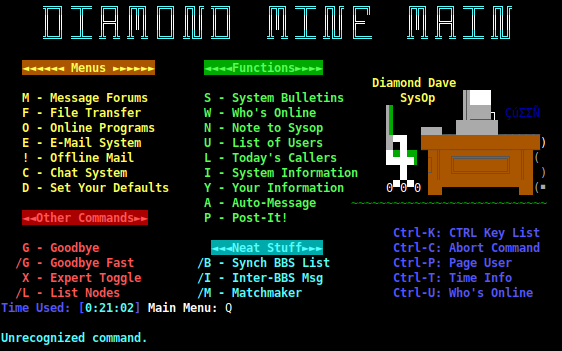
\includegraphics[width=\textwidth]{warez_menu.png}
	\end{center}
\end{frame}

\begin{frame}
	\frametitle{Bulletin Board Systems - Messages}

	\begin{center}
	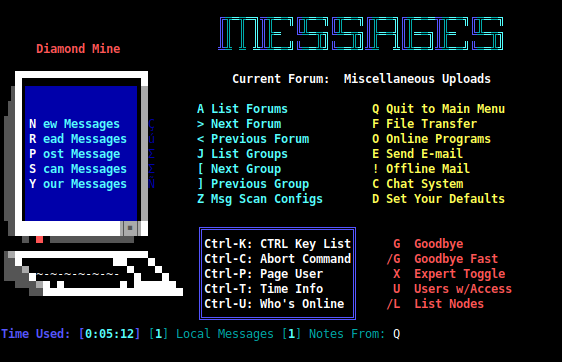
\includegraphics[width=\textwidth]{warez_messages.png}
	\end{center}
\end{frame}

\begin{frame}
	\frametitle{Bulletin Board Systems - Games}

	\begin{center}
	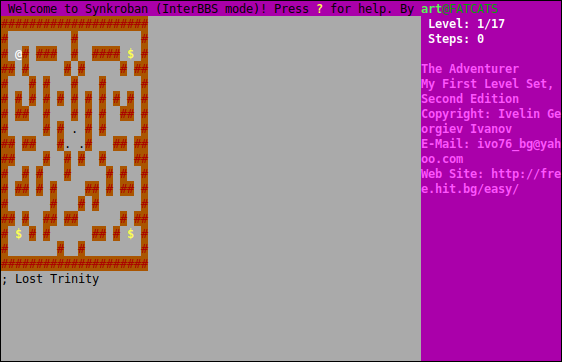
\includegraphics[width=\textwidth]{warez_sokoban.png}
	\end{center}
\end{frame}

\subsection{Demo(scene)}

\begin{frame}
	\frametitle{Demoscene}

	\begin{itemize}
	\item Copyparties
	\item Demos waren beter dan het spel zelf
	\item Groepen gingen demowedstrijden houden
	\end{itemize}
\end{frame}

\begin{frame}
	\frametitle{Demoscene}

	%Oude prod. Evt. bekende prod?
	\begin{center}
	
\includegraphics[width=0.9\textwidth]{second_reality.png}
	\end{center}
	% of juist iets anders voor de verandering? plasma is ook wel cool in de demo
\end{frame}

% future crew: second reality
% farbrausch: fr-041 debris
% chaos theory? http://www.pouet.net/prod.php?which=75713

\begin{frame}
	\frametitle{Demoscene}
	\framesubtitle{Assembly 2004}

	\begin{center}
	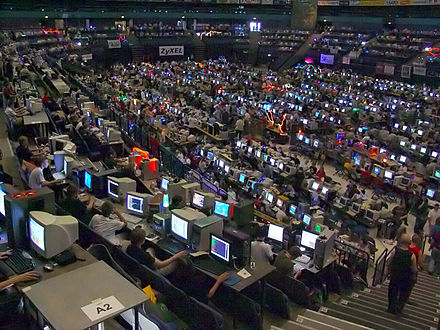
\includegraphics[width=0.9\textwidth]{assembly2004.jpg}
	\end{center}
\end{frame}

\begin{frame}
	\frametitle{Demoscene}
	\framesubtitle{Revision 2015}

	\begin{center}
	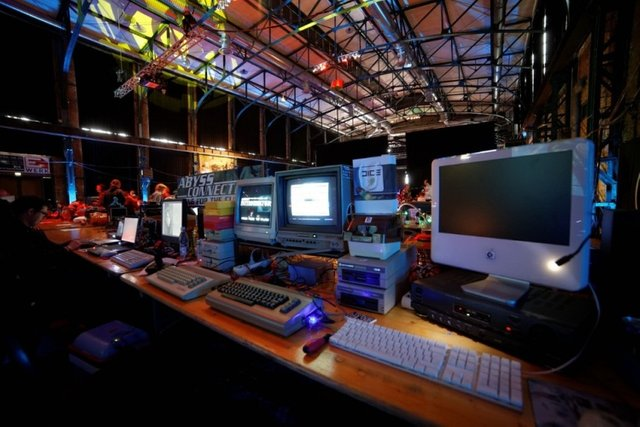
\includegraphics[width=\textwidth]{revision2015.jpeg}
	\end{center}
\end{frame}

\begin{frame}
	\frametitle{Demoscene}
	\framesubtitle{Assembly 2017}

	\begin{center}
	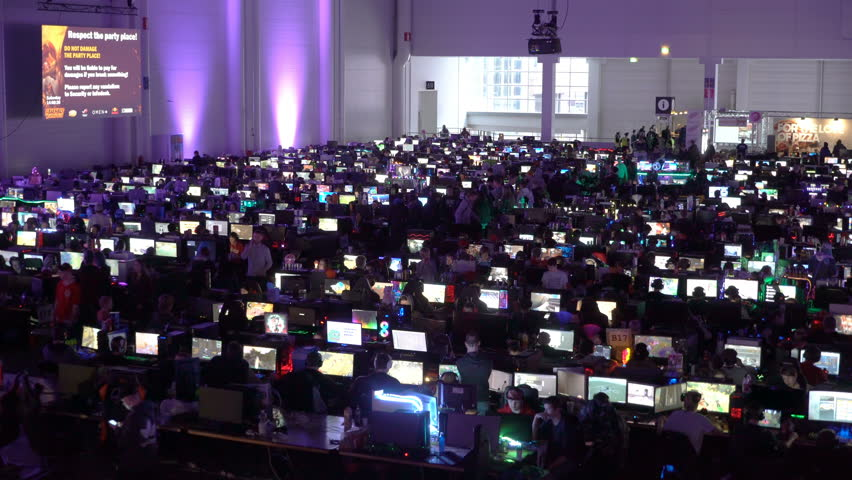
\includegraphics[width=\textwidth]{assembly2017.jpg}
	\end{center}
\end{frame}

\begin{frame}
	\frametitle{Demoscene}

	Nieuwe prod
\end{frame}

% pauze

\begin{frame}
	\frametitle{Lezingencommissie}

	\begin{itemize}
		\item Organiseert educatieve lezingen en workshops van diverse sprekers en studenten
		\item Lezingennieuwsbrief (aanmelden via lezingen@svia.nl)
		\item Ge\"interresseerd? Spreek ons aan of mail naar lezingen@svia.nl
		\item Colloquiumpunten!
	\end{itemize}
\end{frame}

\section{Cracking}
\subsection{Reverse Engineering}
\subsection{API Hacking/spoofing, \dots}

\begin{frame}
	\frametitle{Cracking}

	\begin{itemize}
		\item Key reuse (keygen)
		\item Debugging/Reverse engineering
		\item Emulation of protection schemes
		\item Firmware analysis
		\item API hijacking/spoofing
		\item Patching integrity checks
	\end{itemize}
\end{frame}

\begin{frame}
	\frametitle{Timestopper}

	\begin{center}
	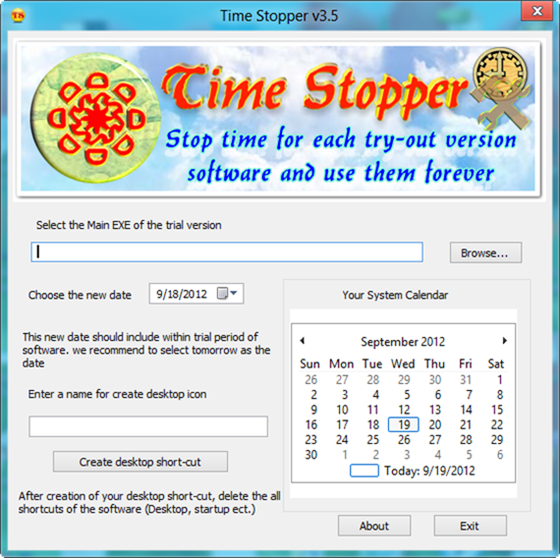
\includegraphics[width=0.75\textwidth]{Time-Stopper.png}
	\end{center}
\end{frame}

% past niet echt in het thema, maar kan er wel bij...
\begin{frame}
	\frametitle{WinRAR}

	Free trial edition
\end{frame}

\begin{frame}
	\frametitle{Gameshark}

	\begin{itemize}
		\item Hexcode
		\item Verschillende standaarden (afh. van platform)
		\item Vervangen van code of data van spel
		\item Code en data op oude hardware op vaste addressen, dus makkelijk aan te passen
		\item Bijv.: levens=5, tijd=999 (dus onbeperkt aantal levens en tijd)
	\end{itemize}
\end{frame}

\begin{frame}
	\frametitle{Debugging/Reverse engineering}

	\begin{itemize}
		\item Gameshark in het kwadraat
		\item Volledige controle over programmaflow
		\item Tijdrovend, maar effectief
		\item Patches/trainers/cracktro's etc.
	\end{itemize}
\end{frame}

% game doctor demo?
% gameshark/cheat engine achtig iets
% VBA demo
% ida free/pro (ghidra? wel van nsa maar ja...)
% timestopper (kan ook aan begin)

\section{Preventie}
\subsection{Detectiesoftware, undocumented `features', \dots}
\subsection{Digital Rights Management}

\begin{frame}
	\frametitle{Prevention}


	\begin{itemize}
		\item Zowel in software als hardware.
		\item Later: Digital Rights Management
		\item \dots
	\end{itemize}
\end{frame}

\begin{frame}
	\frametitle{Prevention - Software en hardware hacks}

	\begin{itemize}
		\item \url{https://www.youtube.com/watch?v=Qaq9vlfoGnA}
		\item Beschadigen van opslagmedium
		\item Debugger detection in leander
		\begin{itemize}
			\item Programma stopt
			\item Programma verandert subtiel dingen (leander)
		\end{itemize}
	\end{itemize}
\end{frame}

\begin{frame}
	\frametitle{Prevention - Lockout}

	\begin{center}
	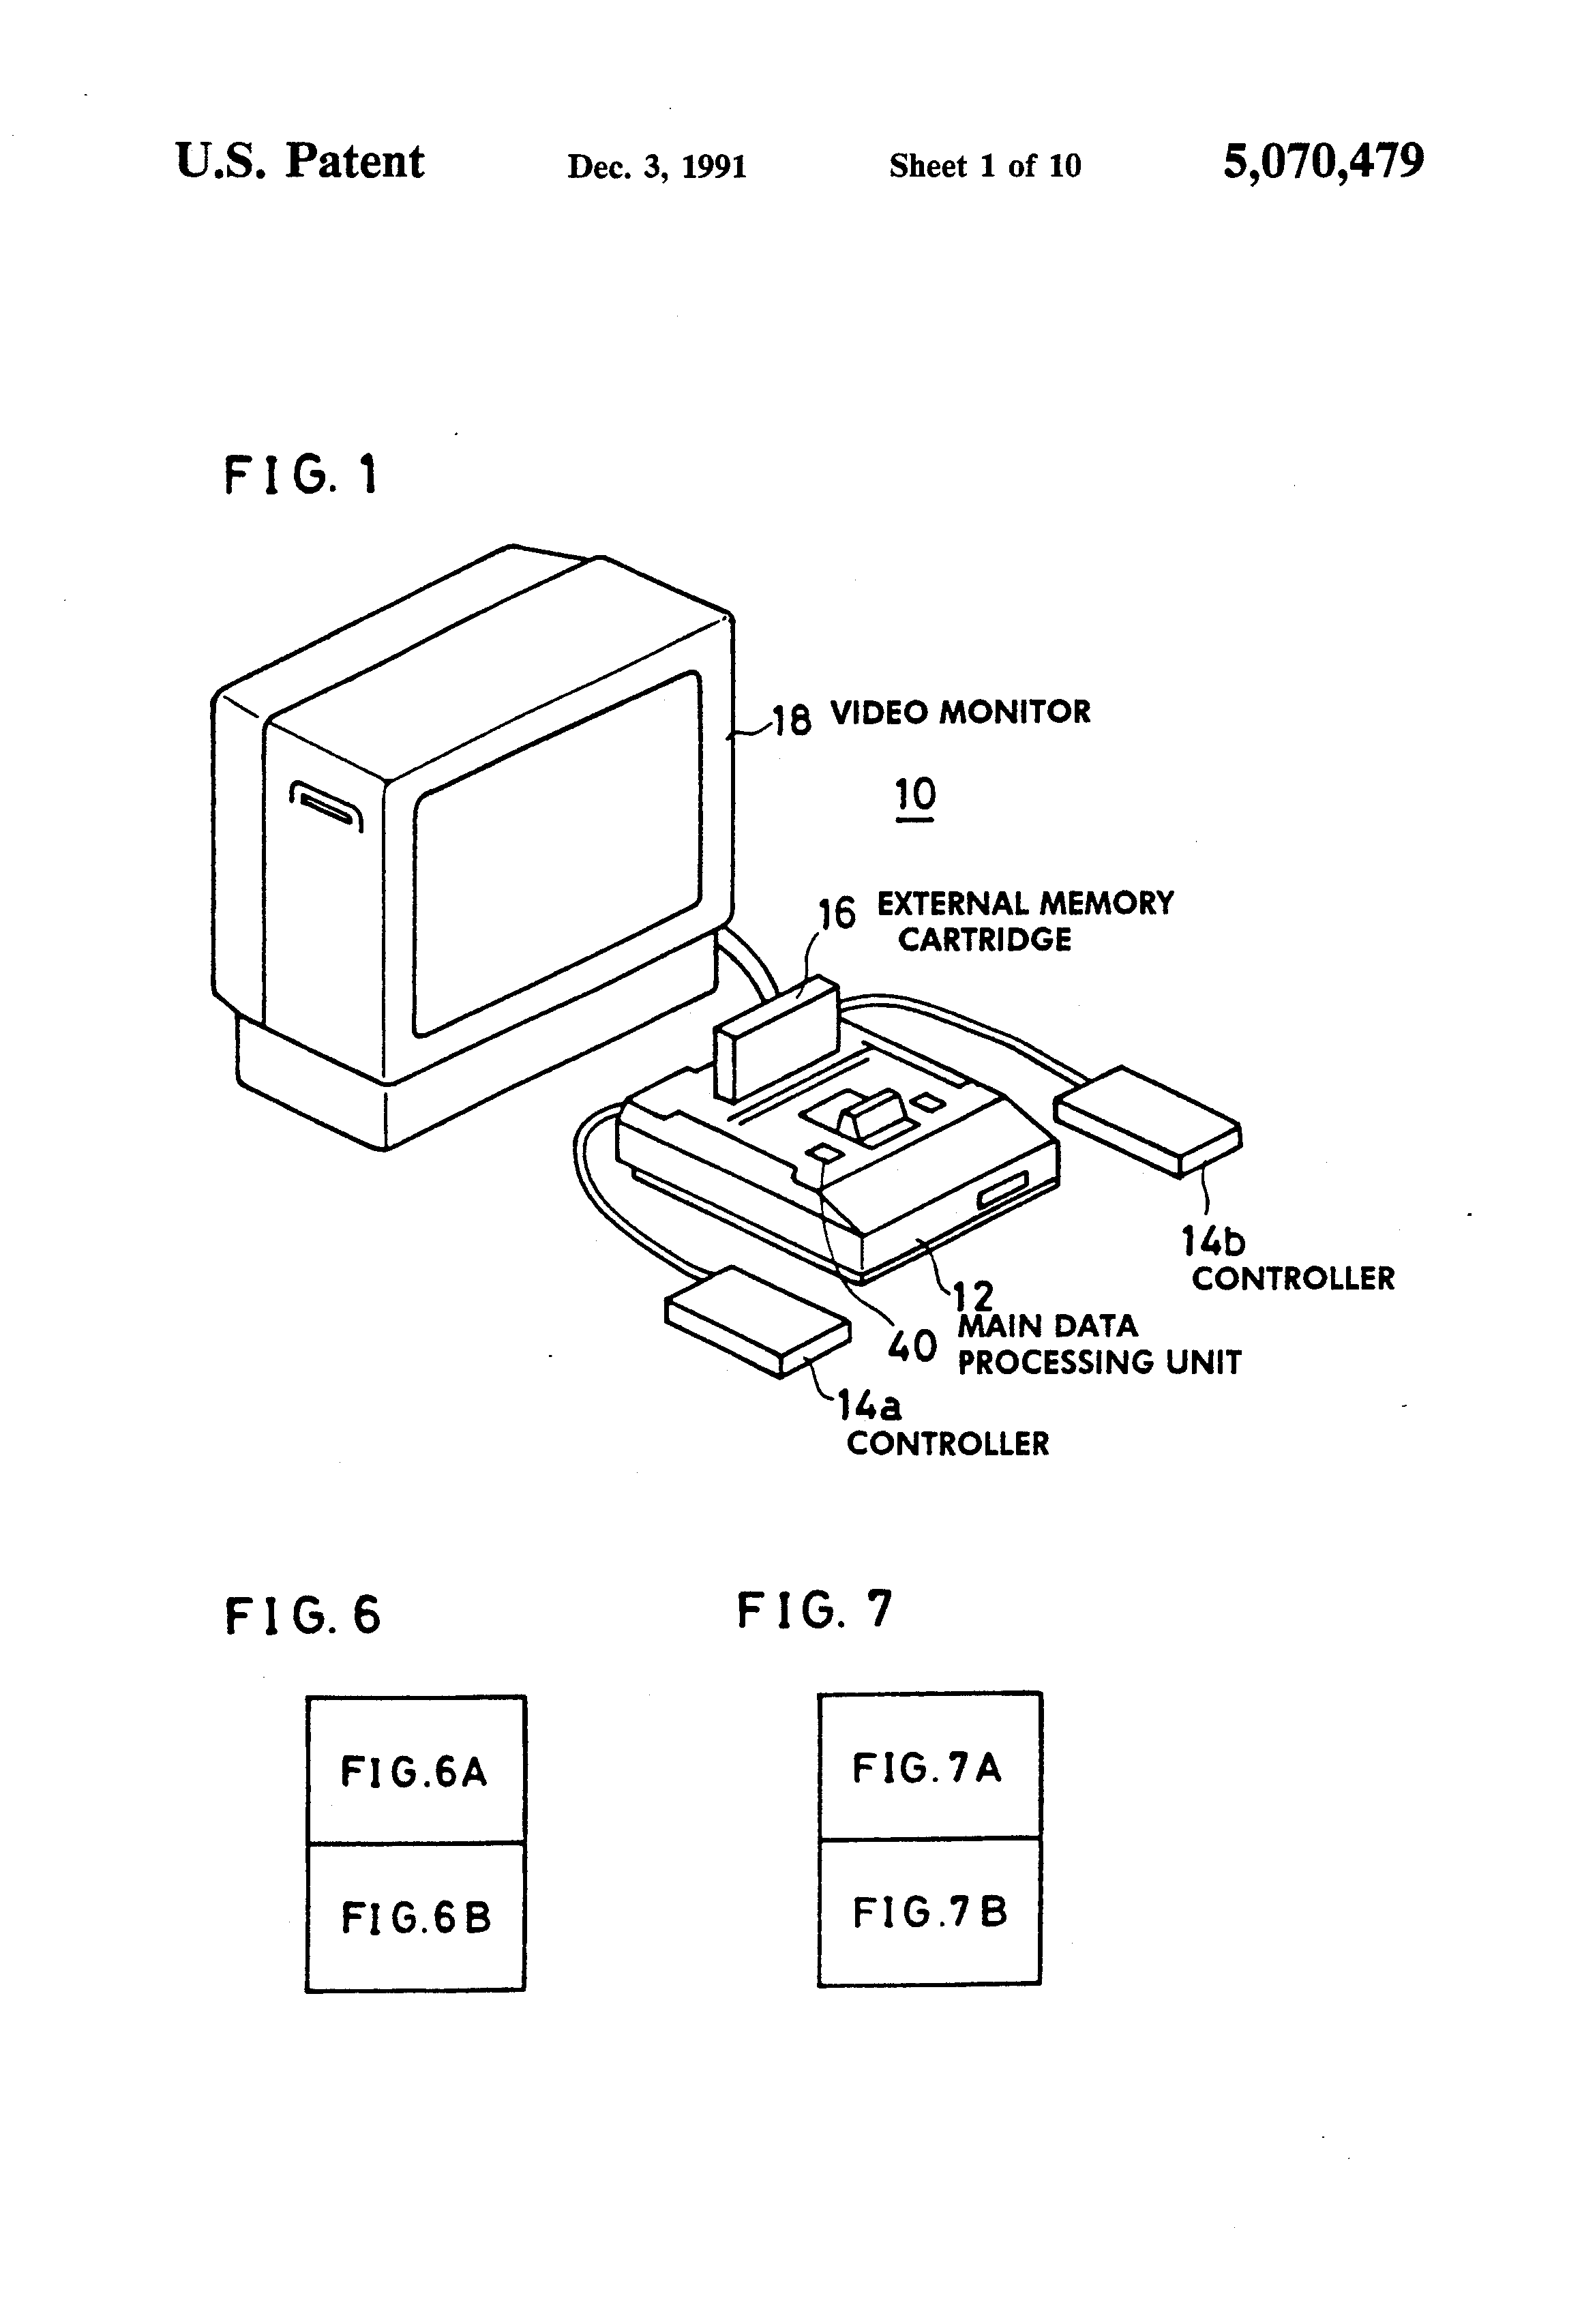
\includegraphics[width=0.6\textwidth]{US5070479-drawings-page-2.png}
	\end{center}
\end{frame}

\begin{frame}
	\frametitle{Prevention - Lockout}

	\begin{center}
	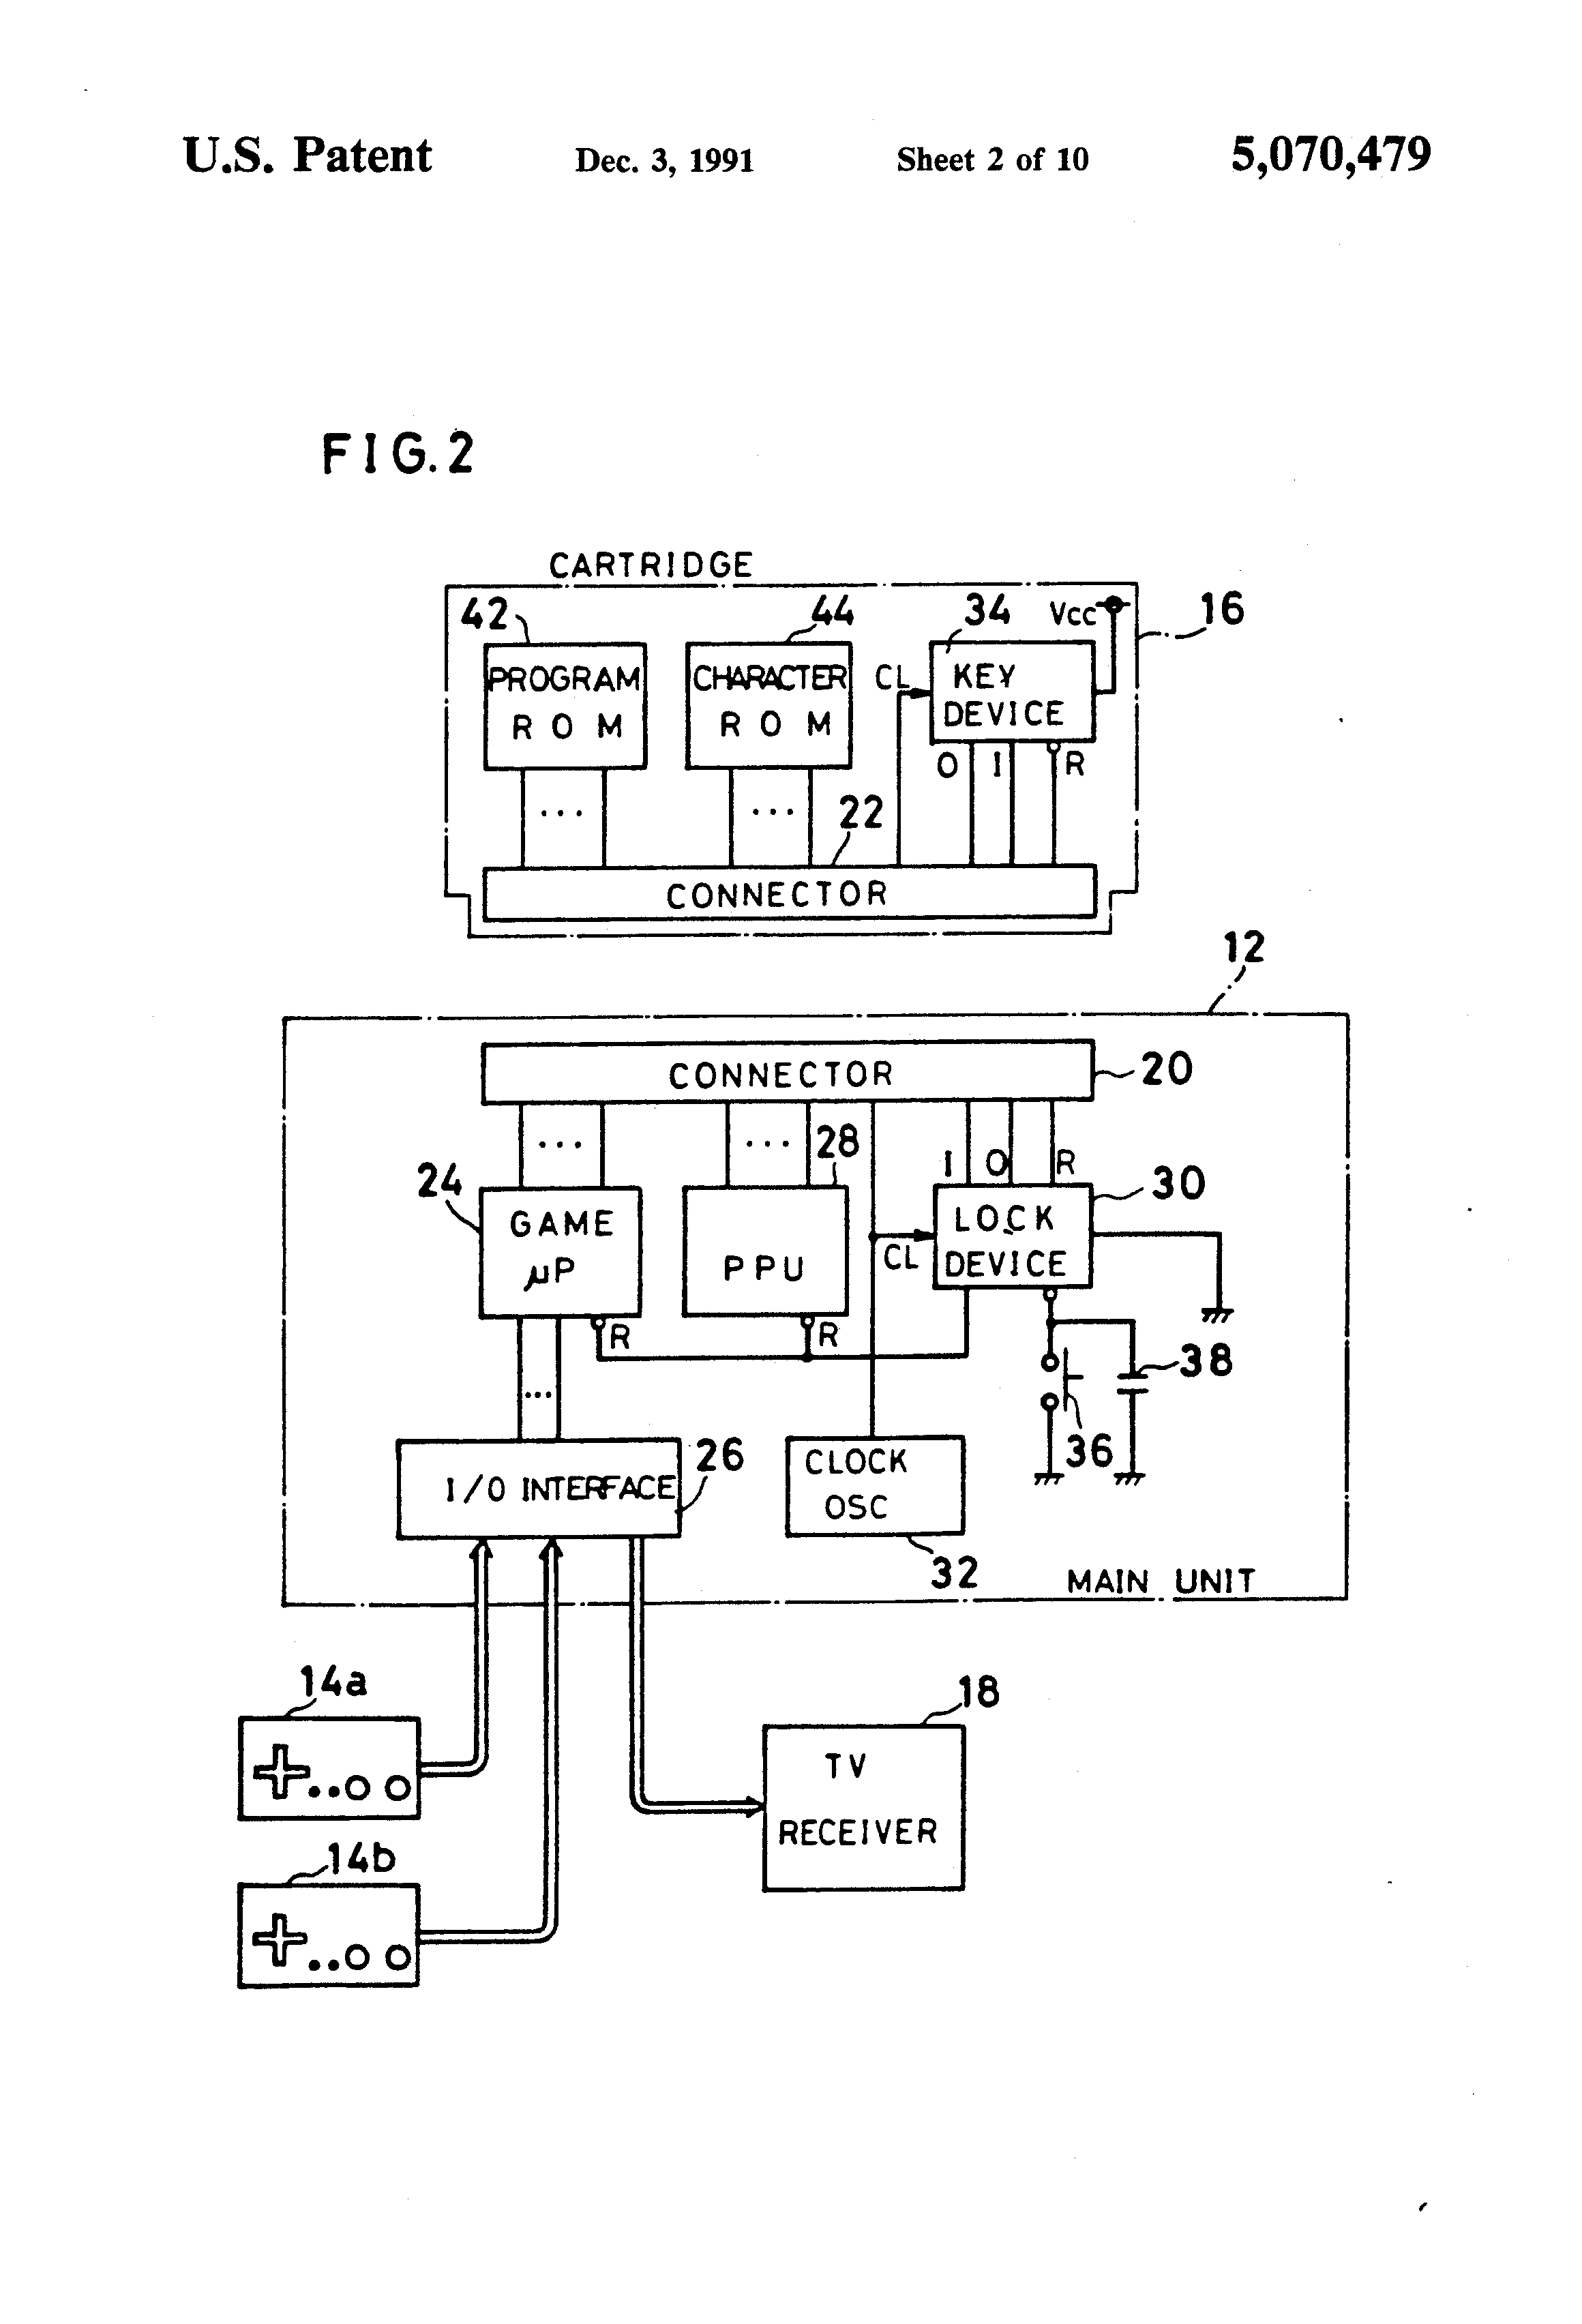
\includegraphics[width=0.6\textwidth]{US5070479-drawings-page-3.png}
	\end{center}
\end{frame}

\begin{frame}
	\frametitle{Prevention - Lockout}

	\begin{center}
	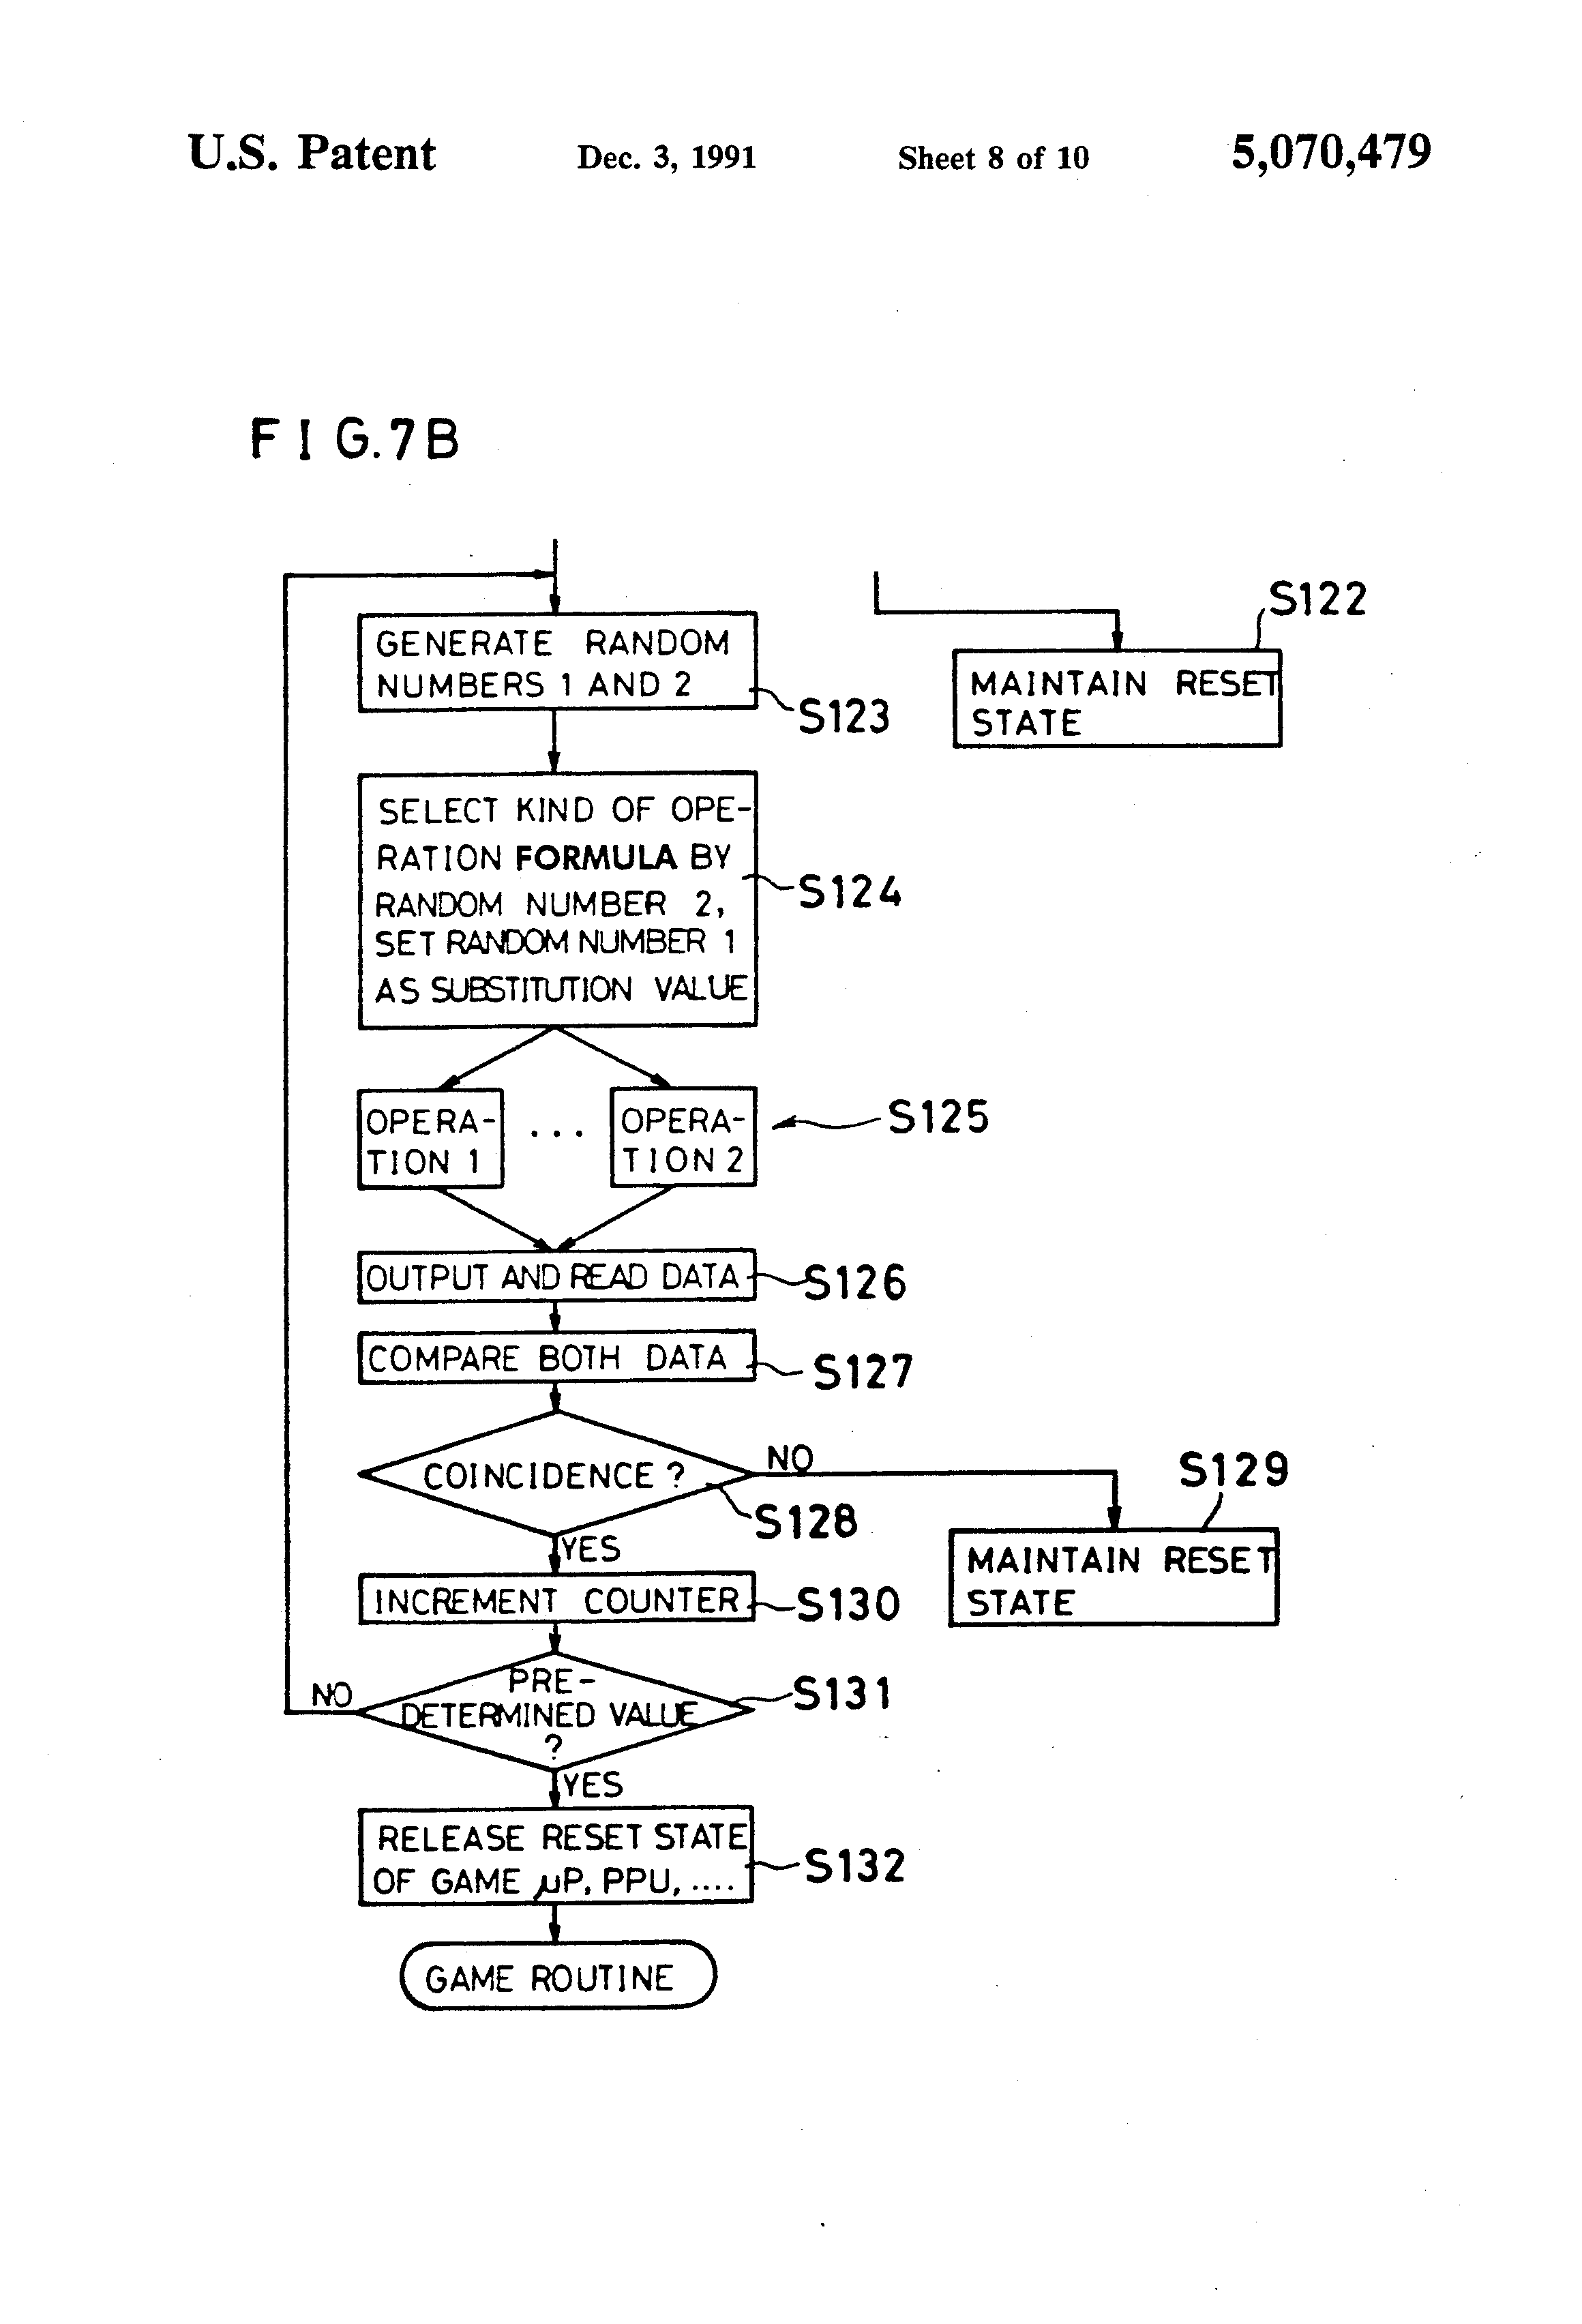
\includegraphics[width=0.6\textwidth]{US5070479-drawings-page-9.png}
	\end{center}
\end{frame}

\begin{frame}
	\frametitle{Prevention}

	\begin{itemize}
		\item Debugger/Emulator detection
		\item Stack smashing
		\item Undocumented opcode/trap
		\item Subtle in-game changes
		\item Opslagmedium beschadigen
		\item Digital Rights Management
		\item Lock-out chips
		\item European Union: `thuisheffingskopiebelasting' (ofwel `piracy tax')
	\end{itemize}
\end{frame}

% plaatje van gaatje in disk zoeken (of maken...)
% tim kuik controversy
% lock-out chips NES, N64 etc. en omzeilen daarvan
% stack smashing voorbeeld? wrs te technisch
% digital restrictions management. sony malware controversy


% etc
\end{document}

